\documentclass[tikz]{standalone}
\usetikzlibrary{positioning}

\newcommand{\po}[2]{\draw [->, thick] (#1) to node[above] {\Large{so}} (#2);}
\newcommand{\povis}[2]{\draw [->, thick] (#1) to node[above] {\Large{so}$,$ \Large{vis}} (#2);}
%p\newcommand{\povis}[2]{\draw [->, thick] (#1) to node[above] {\Large{so}} node[below] {\Large{vis}} (#2);}
\newcommand{\vis}[2]{\draw [->, thick, dashed] (#1) to node[above, sloped, near end] {\Large{vis}} (#2);}
\newcommand{\ar}[2]{\draw [->, thick, dotted] (#1) to node[above, sloped] {\Large{ar}} (#2);}
\newcommand{\vvis}[2]{\draw [->, thick, dashed, allow upside down] (#1) to node[above, sloped] {\Large{vis}} (#2);}

\begin{document}
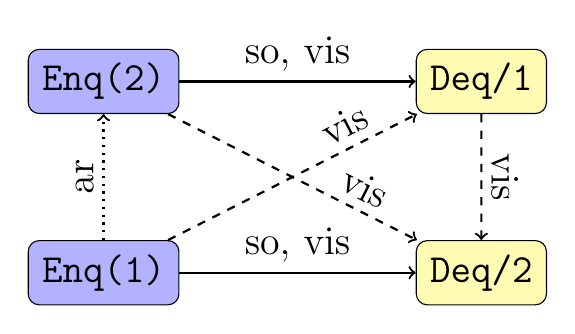
\begin{tikzpicture}
\tikzset{
  enq-op/.style = {rectangle, rounded corners, fill = blue!30, draw, font = \Large, inner sep = 5pt},
  deq-op/.style = {rectangle, rounded corners, fill = yellow!30, draw, font = \Large, inner sep = 5pt},
  process/.style = {font = \huge},
  po/.style = {->, very thick},
  vis/.style = {->, shorten >= 3pt, very thick, dashed}
}

  \node (p1-enq2) [enq-op] {\texttt{Enq(2)}};
  \node (p1-deq1) [deq-op, right = 3cm of p1-enq2] {\texttt{Deq/1}};

  \node (p2-enq1) [enq-op, below = 1.6cm of p1-enq2] {\texttt{Enq(1)}};
  \node (p2-deq2) [deq-op, right = 3 of p2-enq1] {\texttt{Deq/2}};

  \povis{p1-enq2}{p1-deq1};
  \povis{p2-enq1}{p2-deq2};

  \vis{p2-enq1}{p1-deq1};
  \vvis{p1-deq1}{p2-deq2};
  \vis{p1-enq2}{p2-deq2};

  \ar{p2-enq1}{p1-enq2};
\end{tikzpicture}
\end{document}
